\chapter{Einleitung}
\section{Infrastrukturen zur Open Source Softwareentwicklung}
Infrastrukturen zur Open Source Softwareentwicklung war eine Veranstaltung von Steffen Evers an der Technischen Universit"at Berlin im Wintersemester 2005/2006.

Der Inhalt dieser Veranstaltung wird auf der Projekt-Homepage wie folgt beschrieben:

\textit{Ein derartiger Entwicklungsprozess ist von der genutzten technischen Infrastruktur sehr abh�ngig. Wir werden daher verschiedene Werkzeuge und Plattformen untersuchen, weiterentwickeln und auch neue, unterst�tzende Systeme bauen.}

\section{TeamFound}
\begin{figure}[h]

\epsfig{file=logo_teamfound}
\caption{TeamFound Logo}
\label{logo}
\end{figure}
TeamFound ist wie man bereits aus dem Namen schliessen mag eine Suchmaschine f�r Teams. Der Vorteil einer eigenen Suchmaschine liegt ganz einfach darin, das nicht jedes Teammitglied eine herk�mmliche Suchmaschine bem�hen muss um Inhalte zu finden, die ein anderes Teammitglied bereits recherchiert hat. Andererseits ist es aber nicht gesagt, das die gesuchten Informationen wirklich schon in der eigenen Teamsuchmaschine vorhanden ist, daher suchen TeamFound-Clients immer auch in einer zweiten herk�mmlichen Suchmaschine.

Bisherige Technik um Suchergebnisse zu verteilen integrieren sich dagegen sehr viel schlechter in einen vorhandenen Arbeitsprozess, zum Beispiel k�nnten einfache Bookmarks ausgetauscht werden, diese sind aber unter Umst�nden nicht von allen Teammitgliedern ver�nderbar, die Integration in einen Webbrowser ist hier quasi nicht vorhanden. 

Eine weitere M�glichkeit bieten Kataloge\footnote{Jede gr��ere Suchmaschine bietet eigene Kataloge. Das DMOZ-Projekt (http:/www.dmoz.org) stellt einen unabh�ngigen Versuch dar, das Internet zu kategorisieren} oder Verschlagwortungen wie del.icio.us \footnote{http://del.icio.us}, selbst wenn eine derartige Software in Form einer Teamsuchmaschine eingesetzt werden k�nnen, bieten sie eigentlich keine Integration in vorhandene Browser und damit w�rden vorhandene Arbeitsabl�ufe nachhaltig gest�rt.
\\
TeamFound will - gerade durch die Integration in bekannte Browser - diese Integration einfacher m�glich machen. Das Hinzuf�gen neuer Seiten sowie das Suchen im eigenen Index ist durch eine einfache Toolbar oder - genau wie bei bekannten Suchmaschinen - mittels einer Webseite m�glich. Dabei k�nnen Seiten nicht nur in den Index eingef�gt werden sondern auch in beliebig viele Kategorien einsortiert werden, welche wiederrum einzeln oder als Baum durchsucht werden k�nnen.

\subsection{Komponenten}

\begin{figure}[h]
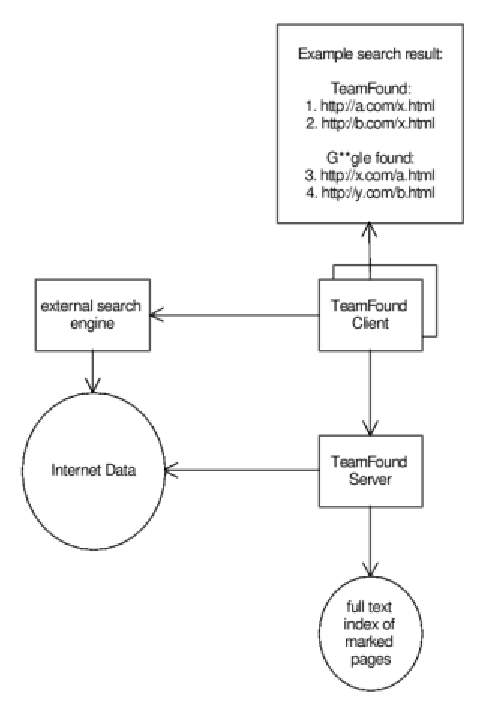
\epsfig{file=architecture1}
\caption{grobe Architektur Client - Server - Suchmaschiene}
\label{webclient}
\end{figure}

TeamFound besteht aus mehreren Komponenten, zentraler Bestandteil ist wie bei allen anderen vorgestellten Technologien ein Server, welche Suchanfragen entgegennimmt, deren Ergebnisse �bermittelt und sich au�erdem um das herunterladen neuer Seiten und deren einf�gen in den Index k�mmert. Anders als bei anderen Technologien, ist die Client-Integration aber seit Beginn des projektes Teil der Planungen. TeamFound implementiert Clients unter anderem als Toolbar in bekannte Browser, nat�rlich ist es auch f�r ein geeignetes Webfrontend m�glich TeamFound-Server zu benutzen, genauso wie auch andere Suchmaschinen meist �ber deren Internetseiten benutzt werden. Allerdings wurde bei der Clientkonzeption von TeamFound eher auf die M�glichkeiten von Browsererweiterungen eingegangen, als auf die Anforderungen von Webseiten.

Im Folgenden werden die einzelnen Teile von TeamFound detailliert dargestellt. Dabei handelt es sich zuerst um den TeamFound-Server und anschliessend um die Toolbars f�r den Firefox-Browser vom Mozilla-Projekt sowie der Integration in den Internet Explorer von Microsoft. Da diese Browser auf sehr unterschiedlicher Technik basieren werden die einzelnen Toolbars auch getrennt beschrieben.

\subsection{Funktionsumfang}

\subsubsection{Suchanfragen}

Suchanfragen an TeamFound werden wie in jeder anderen Volltextsuche mittels Schl�selw�rter gestellt. Dabei h�ngt es von der Index-Implementierung ab, wie genau verschiedene Felder durchsucht oder Schl�sselw�rter verkn�pft werden k�nnen.

\subsubsection{Kategorien}
\label{kategorien}
Jedes Dokument im Index kann in einer oder mehrerer Kategorien enthalten sein. Kategorien werden dabei als Baum dargestellt, es gibt also eine Wurzelkategorie sowie eine unbestimmte Anzahl weiterer Kategorien die jeweils eine Elternkategorie haben. 

Suchanfragen an eine Kategorie findet nur Dokumente in dieser oder einer ihrer Unterkategorien. Das wirkliche Begrenzen der Suche auf genau eine Kategorie, ohne Unterkategorien ist in dieser TeamFound-Version noch nicht vorhanden.


